% =====================================================================
% Foresight model paper (IEEE conference format). All numbers come from
% releases/final_review/data/all_facts.json and artifacts/experiments/*.
% Replace the author block before submission.
% Compile: tectonic Foresight_Model_Paper.tex
% =====================================================================
\documentclass[conference]{IEEEtran}
\usepackage[T1]{fontenc}
\usepackage{amsmath,amssymb}
\usepackage{graphicx}
\usepackage{booktabs}
\usepackage{url}
\usepackage[hidelinks]{hyperref}
\graphicspath{{../final_review/figures/}}

\begin{document}

\title{Foresight: Leakage-Controlled Vision Transformer for Visual Produce-Spoilage Estimation with Human-Validated Decay Labels}

% TODO: replace with real author names, affiliations and e-mails.
\author{\IEEEauthorblockN{Author One, Author Two, Author Three}
\IEEEauthorblockA{Department, Institution, City, Country\\ \{author1, author2, author3\}@institution.edu}}

\maketitle

\begin{abstract}
Image-based spoilage classifiers are often evaluated on random splits of datasets that contain duplicate images and repeated views of the same specimen, which inflates reported accuracy.
We present Foresight, a single-photo produce-spoilage estimator built on the public TriModal Ripeness~6 (TR-6) dataset.
An audit showed that all 10,796 \emph{Classified} images are byte-identical copies of \emph{Normal} images, and that 170 contents carry contradictory labels.
After de-duplication, we split 5,335 eligible sRGB images 60/20/20 by capture session.
A fine-tuned ViT-B/16 reaches a test spoilage macro-F1 of 0.954 (95\% session-bootstrap CI 0.903--0.988), ROC-AUC 0.989, and 100\% produce-type accuracy.
Controlled three-seed ablations show three effects:
\begin{itemize}
\item conventional augmentation gives a small but consistent gain (+0.013);
\item class-conditional GAN augmentation gives no reliable gain;
\item evaluating on unseen capture days lowers macro-F1 by 0.098.
\end{itemize}
A human review of 165 images found visible decay in only 72 of 109 images labelled \emph{Spoiled}. This shows that the dataset label partly encodes storage time rather than visible decay.
The model is deployed in a tested FastAPI/React application with three further outputs, each labelled in the app as what it is: attention-rollout explanations, a visible-decay check trained on human labels, and pilot segmentation and proxy shelf-life outputs.
\end{abstract}

\begin{IEEEkeywords}
Food spoilage, vision transformer, data leakage, explainable AI, GAN augmentation, dataset auditing.
\end{IEEEkeywords}

\section{Introduction}
Post-harvest loss of fruit and vegetables is a major contributor to food waste. Visual inspection is the most common triage method but is subjective.
Deep image classifiers can automate this triage. However, their reported accuracies depend heavily on how training and test images are separated.
When a dataset contains repeated views of the same specimen, a random split places near-identical images in both partitions, and the test score then measures memorisation rather than generalisation.

This paper studies spoilage estimation on TR-6~\cite{tr6} with an emphasis on evaluation validity. Our contributions are:
\begin{enumerate}
\item an audit of TR-6 that quantifies duplicate and same-session leakage under different split strategies;
\item a fine-tuned vision transformer~\cite{vit} evaluated on a duplicate-aware, session-grouped split, with bootstrap confidence intervals;
\item controlled multi-seed ablations of augmentation, GAN augmentation~\cite{dcgan,cgan}, split design, noise robustness and denoising~\cite{dncnn};
\item a human validation of the dataset's spoilage labels;
\item an integrated, tested application that labels pilot and proxy outputs as such.
\end{enumerate}

\section{Dataset and Leakage Control}
TR-6 contains 21,653 files (19.8~GiB): 10,676 sRGB images, 10,950 thermal IR-fusion images and 18 methane logs. They cover six produce types: banana, carrot, guava, Indian gooseberry, mango and tomato. Each fruit was photographed from 17 viewpoints per capture session over consecutive days.

\textbf{Audit.} Hashing every file with SHA-256 yields only 10,776 unique image contents, because the \emph{Classified} tree is a relabelled copy of the \emph{Normal} tree. 170 contents (all thermal) appear under both labels. Within every produce type, all \emph{Not spoiled} captures precede all \emph{Spoiled} captures.

\textbf{Eligibility and split.}
\begin{itemize}
\item Conflicting contents were excluded rather than tie-broken. \emph{Normal}-only contents were treated as unlabelled.
\item Only sRGB was used, because the target application receives phone photographs. This left 5,335 eligible images.
\item A capture session was defined as images of the same produce and label taken at most 300\,s apart. Sessions were assigned 60/20/20 within each produce\,$\times$\,label stratum (seed 42), giving 3,177/1,087/1,071 images and 189/64/64 sessions.
\end{itemize}

Table~\ref{tab:leak} shows why this matters. A random split of the raw files places an exact copy of 59.8\% of test images in training, and a same-session view of every test image. The session split removes both kinds of leakage, but 76.2\% of test images still share a produce and capture day with training. A day-grouped variant reduces that to 1.5\% and is used as a sensitivity test.

\begin{table}[t]
\caption{Test-to-train leakage under different split strategies}
\label{tab:leak}
\centering\footnotesize
\begin{tabular}{@{}lrrr@{}}
\toprule
Split strategy & Exact dup. & Same session & Same day \\
\midrule
Random, raw files & 59.8\% & 100.0\% & 100.0\% \\
Random, de-duplicated & 0.0\% & 99.9\% & 100.0\% \\
Session-grouped (ours) & 0.0\% & 0.0\% & 76.2\% \\
Day-grouped (sensitivity) & 0.0\% & 0.0\% & 1.5\% \\
\bottomrule
\end{tabular}
\end{table}

\section{Method}
\textbf{Model.} We fine-tune a ViT-B/16 pretrained on ImageNet-21k and ImageNet-1k (86\,M parameters, \texttt{timm}~\cite{timm}). Two linear heads act on the CLS embedding $z$:
\begin{equation}
p_{\text{type}}=\mathrm{softmax}(W_t z+b_t),\qquad p_{\text{spoil}}=\mathrm{softmax}(W_s z+b_s).
\end{equation}
The loss is $\mathcal{L}=\mathrm{CE}(y_t,p_{\text{type}})+\mathrm{CE}(y_s,p_{\text{spoil}})$. Self-attention follows $\mathrm{softmax}(QK^\top/\sqrt{d_k})V$.

\textbf{Training.}
\begin{itemize}
\item Optimiser: AdamW with weight decay 0.01, a backbone learning rate of $2\times10^{-5}$ and a head learning rate of $2\times10^{-4}$, one warm-up epoch and cosine decay.
\item Schedule: batch 16, 12 epochs, 224$\times$224 input.
\item Augmentation: crop, flips, $\pm15^\circ$ rotation and $\pm0.15$ brightness/contrast. Hue and saturation are left unchanged so that colour cues of decay are preserved.
\item Selection: the checkpoint is chosen by validation composite macro-F1 (epoch 9 of 12), and the test set is scored once.
\item Hardware: training took 54.7\,min on an Apple M5 GPU (MPS).
\end{itemize}

\textbf{Explanations.} Attention rollout~\cite{rollout} multiplies head-averaged, residual-corrected attention matrices across the 12 blocks.

\textbf{Additional outputs.} Three lightweight models reuse the frozen embedding $z$ or the image:
\begin{enumerate}
\item a logistic \emph{visible-decay} probe trained on human labels (Section~\ref{sec:human});
\item a ridge regressor for a \emph{proxy} shelf-life, defined as the days until the series' first \emph{Spoiled} capture;
\item a pilot U-Net~\cite{unet} with a ResNet-18 encoder~\cite{resnet} for fruit and decay masks, trained with $0.5\,\mathrm{BCE}+0.5\,\mathrm{Dice}$ on machine-generated masks.
\end{enumerate}

\section{Results}
\textbf{Main result.} On the 1,071 test images the deployed model achieves:
\begin{itemize}
\item spoilage accuracy 0.961, macro-F1 0.954 and ROC-AUC 0.989;
\item a session-level bootstrap 95\% CI for macro-F1 of 0.903--0.988;
\item 100\% produce-type accuracy (Fig.~\ref{fig:cm}).
\end{itemize}
The \emph{Spoiled} class has precision 0.981 but recall 0.894: 36 of 340 test images are missed, 27 of them Indian gooseberries. The spoilage head has an ECE of 0.038, yet 88\% of its errors are made with confidence of at least 0.9.

\begin{figure}[t]
\centering
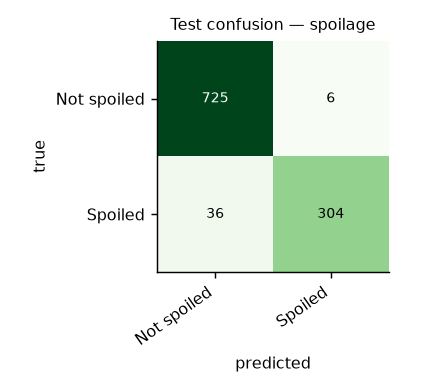
\includegraphics[width=0.48\linewidth]{primary_confusion_spoilage.png}\hfill
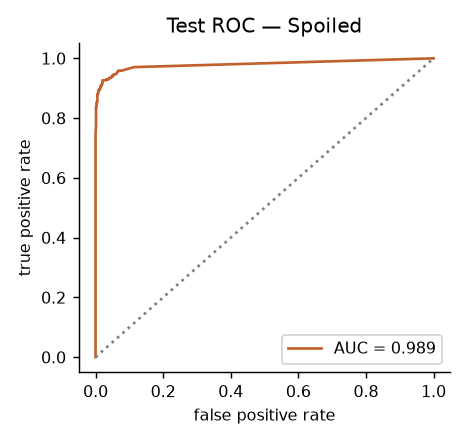
\includegraphics[width=0.48\linewidth]{primary_roc_spoilage.png}
\caption{Test confusion matrix and ROC curve for the spoilage head.}
\label{fig:cm}
\end{figure}

\textbf{Baselines and ablations (Table~\ref{tab:abl}).} Colour-histogram and frozen-ViT linear probes reach macro-F1 0.828 and 0.916. All ViT-S/16 conditions use identical settings and three seeds.
\begin{itemize}
\item Conventional augmentation improves macro-F1 by +0.013, positive on all seeds.
\item Adding 480 GAN images changes it by $-0.009$, with an inconsistent sign across seeds.
\item The GAN images are of limited quality: the real-data classifier recognises the intended produce in only 34.6\% of them. No memorisation was found; the median nearest-neighbour distance is 22.5, against 12.8 between real images.
\item The same configuration evaluated on the day-grouped split loses 0.098 macro-F1 ($0.830\pm0.007$), which shows that session-level results are optimistic for unseen days.
\end{itemize}

\begin{table}[t]
\caption{Test spoilage macro-F1 (ViT-S: mean $\pm$ SD of 3 seeds)}
\label{tab:abl}
\centering\footnotesize
\begin{tabular}{@{}lcc@{}}
\toprule
Model & Macro-F1 & ROC-AUC \\
\midrule
Colour histogram + LogReg & 0.828 & 0.885 \\
Frozen ViT-B/16 + LogReg & 0.916 & 0.979 \\
ViT-S/16, no augmentation & $0.914\pm0.006$ & 0.971 \\
ViT-S/16, conventional aug. & $0.928\pm0.007$ & 0.981 \\
ViT-S/16, conv. aug. + GAN & $0.919\pm0.018$ & 0.976 \\
ViT-S/16, conv. aug., day split & $0.830\pm0.007$ & 0.909 \\
\textbf{ViT-B/16 (deployed)} & \textbf{0.954} & \textbf{0.989} \\
\bottomrule
\end{tabular}
\end{table}

\textbf{Noise robustness (Fig.~\ref{fig:noise}).} With deterministic test corruptions, spoilage macro-F1 drops:
\begin{itemize}
\item to 0.805 under Gaussian noise ($\sigma=0.2$);
\item to 0.776 under salt-and-pepper noise ($p=0.1$);
\item to 0.800 under speckle noise ($\sigma=0.5$).
\end{itemize}
Produce accuracy stays at or above 0.96 in every condition. A 3$\times$3 median filter restores salt-and-pepper performance to 0.934. A resumed DnCNN gives small gains only under heavy noise. The intrinsic noise of TR-6 ($\sigma\approx0.003$) is far below these stress levels.

\begin{figure}[t]
\centering
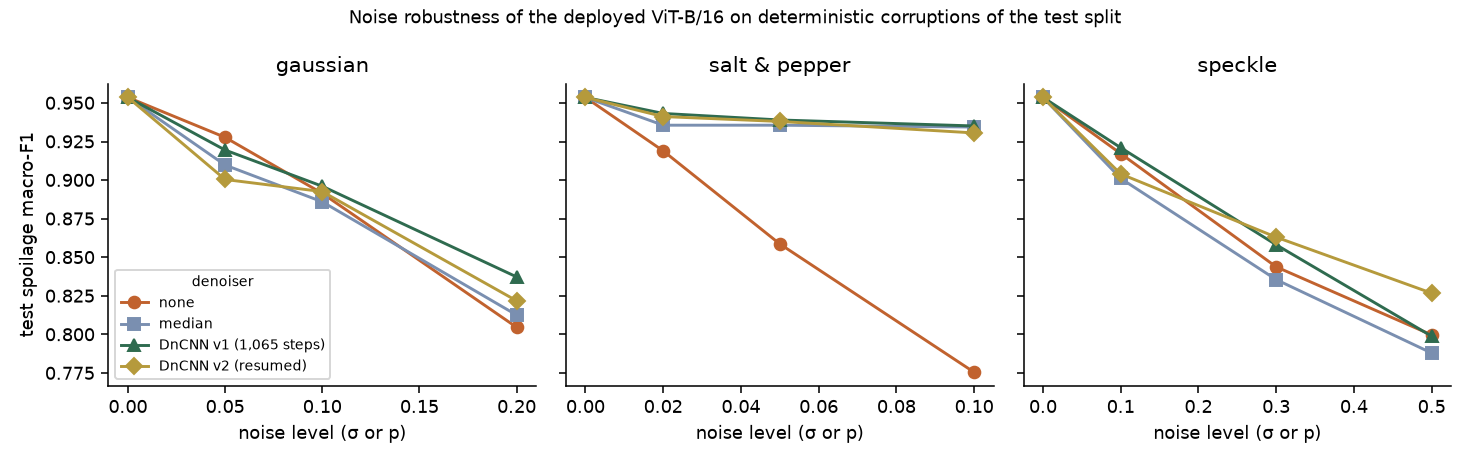
\includegraphics[width=\linewidth]{noise_robustness.png}
\caption{Spoilage macro-F1 under synthetic noise with and without denoising.}
\label{fig:noise}
\end{figure}

\textbf{Explainability.} Rollout maps concentrate on the fruit (Fig.~\ref{fig:xai}).
\begin{itemize}
\item \emph{Faithfulness:} masking the top-20\% rollout patches lowers predicted-class confidence by 0.192, against 0.020 for random patches (Wilcoxon $p=2.3\times10^{-30}$, $n=240$).
\item \emph{Stability:} maps are stable under horizontal flip (Spearman $\rho=0.95$) and mild noise ($\rho=0.96$), against 0.59 between different images.
\item \emph{Artefacts:} isolated bright background tokens match known ViT register artefacts~\cite{registers}.
\item \emph{K-means:} with $k=6$ on frozen ViT embeddings, clusters recover produce type (NMI 0.95) but not spoilage (NMI 0.14).
\end{itemize}

\begin{figure}[t]
\centering
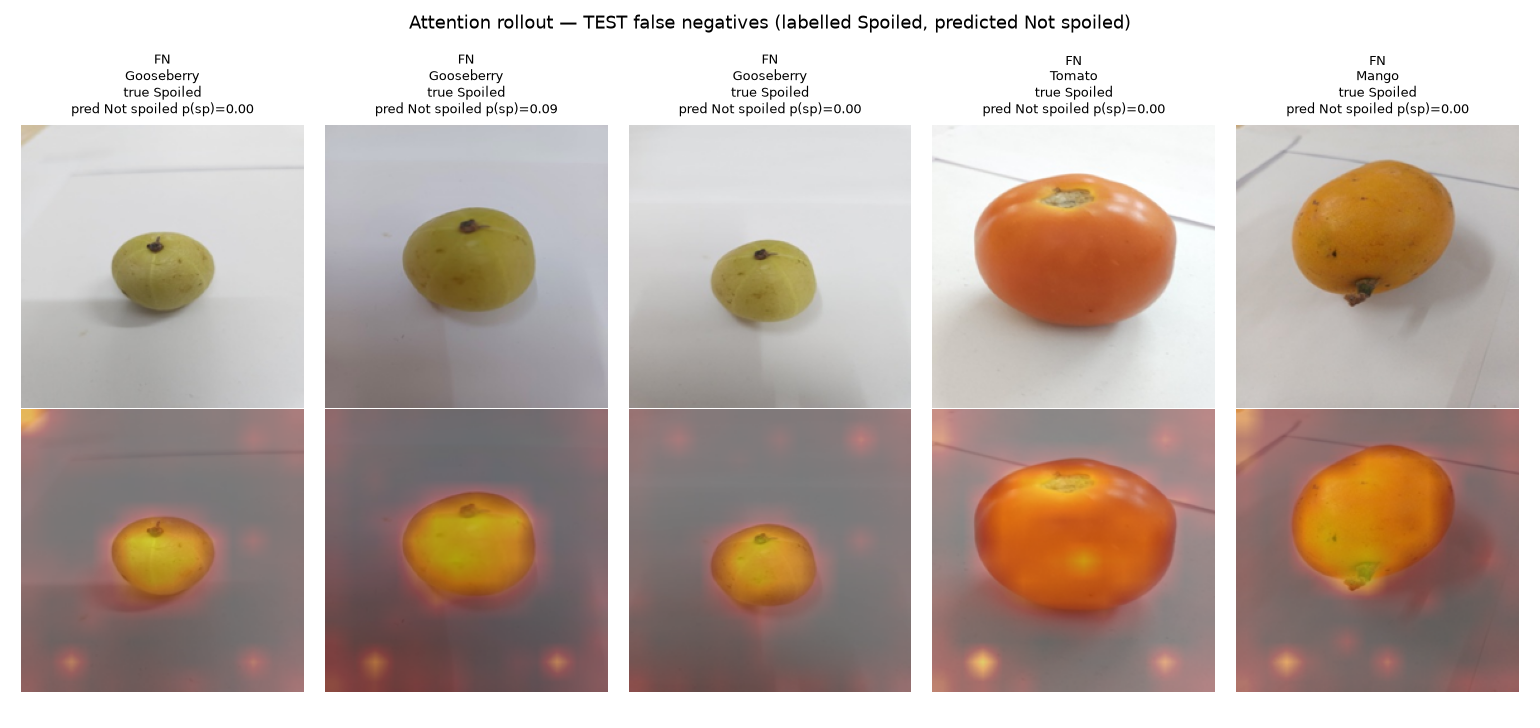
\includegraphics[width=\linewidth]{xai_failure_fn.png}
\caption{Attention rollout on test false negatives: \emph{Spoiled}-labelled fruit without visible decay.}
\label{fig:xai}
\end{figure}

\section{Human Validation of Spoilage Labels}\label{sec:human}
A stratified set of 180 images was reviewed in Label Studio, giving 165 definite decisions.
\begin{itemize}
\item Visible decay was seen in 72 of 109 \emph{Spoiled}-labelled images and in 6 of 56 \emph{Not spoiled} ones, an agreement of 73.9\%.
\item Agreement is high for banana and carrot (20/20 each) but low for tomato (2/20).
\item This explains the model's tomato and gooseberry false negatives: the folder label marks storage time, which can precede visible decay.
\end{itemize}
A visible-decay probe trained on 102 of these decisions reaches 0.931 test accuracy (95\% CI 0.78--0.98, $n=29$; AUC 0.986). Using the spoilage head directly as a decay detector reaches 0.897 accuracy (AUC 0.881).

\section{System and Additional Outputs}
\textbf{Application.} The React UI posts a photo to a FastAPI service, which validates the upload, runs all models and stores the result in SQLite without keeping the image.
\begin{itemize}
\item Median end-to-end latency is 48\,ms on the M5 GPU; a ViT-B forward pass takes 201\,ms on CPU.
\item 37 backend/ML tests and 7 frontend tests pass, and a live end-to-end test passes 11/11 checks.
\item Of 60 held-out full-resolution images, the live API classified produce type correctly for 60 and spoilage for 57.
\end{itemize}

\textbf{Additional outputs.}
\begin{itemize}
\item The proxy shelf-life regressor reaches a test MAE of 4.29 days ($R^2=0.89$), against 9.95 days for a per-produce mean.
\item The pilot U-Net agrees with its machine-generated reference masks with fruit Dice 0.98 and decay Dice 0.59 ($n=63$).
\end{itemize}
Both outputs are labelled as proxy or pilot in the interface. They are not validated against measured shelf life or human-drawn decay masks.

\section{Limitations}
\begin{itemize}
\item \textbf{Specimens:} TR-6 lacks specimen identifiers, so the same physical fruits appear in training and test.
\item \textbf{Domain:} all images are lab photographs on plain backgrounds; real-world photos were not evaluated.
\item \textbf{Labels:} the spoilage labels are date-based.
\item \textbf{Annotation:} the human labels come from a single annotator.
\item \textbf{Seeds:} the deployed model was trained with one seed.
\end{itemize}

\section{Conclusion}
On TR-6, evaluation design matters more than model choice: duplicate-aware, session-grouped splitting is essential, and day-level generalisation remains notably harder.
A fine-tuned ViT-B/16 gives strong, explainable spoilage estimates in a working application.
Human validation shows that the dataset's \emph{Spoiled} label must be interpreted as a storage-stage label.
Future work: human-drawn decay masks for a validated U-Net, real-world test photos, confidence calibration and public deployment.

\begin{thebibliography}{10}
\bibitem{tr6} T.~Bagyammal, Y.~A.~P.~T.~S, K.~Deepak, and D.~Unnikrishnan, ``TriModal Ripeness 6,'' figshare, Dataset, 2025, doi: 10.6084/m9.figshare.30783827.v1.
\bibitem{vit} A.~Dosovitskiy \emph{et al.}, ``An image is worth 16x16 words: Transformers for image recognition at scale,'' in \emph{Proc. ICLR}, 2021.
\bibitem{rollout} S.~Abnar and W.~Zuidema, ``Quantifying attention flow in transformers,'' in \emph{Proc. ACL}, 2020, pp. 4190--4197.
\bibitem{unet} O.~Ronneberger, P.~Fischer, and T.~Brox, ``U-Net: Convolutional networks for biomedical image segmentation,'' in \emph{Proc. MICCAI}, 2015, pp. 234--241.
\bibitem{resnet} K.~He, X.~Zhang, S.~Ren, and J.~Sun, ``Deep residual learning for image recognition,'' in \emph{Proc. CVPR}, 2016, pp. 770--778.
\bibitem{dcgan} A.~Radford, L.~Metz, and S.~Chintala, ``Unsupervised representation learning with deep convolutional generative adversarial networks,'' in \emph{Proc. ICLR}, 2016.
\bibitem{cgan} M.~Mirza and S.~Osindero, ``Conditional generative adversarial nets,'' arXiv:1411.1784, 2014.
\bibitem{dncnn} K.~Zhang, W.~Zuo, Y.~Chen, D.~Meng, and L.~Zhang, ``Beyond a Gaussian denoiser: Residual learning of deep CNN for image denoising,'' \emph{IEEE Trans. Image Process.}, vol.~26, no.~7, pp. 3142--3155, 2017.
\bibitem{registers} T.~Darcet, M.~Oquab, J.~Mairal, and P.~Bojanowski, ``Vision transformers need registers,'' in \emph{Proc. ICLR}, 2024.
\bibitem{timm} R.~Wightman, ``PyTorch image models,'' GitHub repository, 2019. [Online]. Available: \url{https://github.com/huggingface/pytorch-image-models}
\end{thebibliography}

\end{document}
